\chapter{Literature review}
\label{ch:Literature review}
\section{Analysis-based tools for engineers}
The development of finite element analysis (FEA) has resulted in many different, but very similar, software analysis tools. These tools are often too complex and not agile enough to be used for conceptual design. Their use requires a high level of skill, both in connection with the software and in engineering terms. This type of software has been developed for the late design stage, as a tool with which engineers can verify the form. 

 The analysis procedure for this type of software is often a step-by-step workflow, where all the steps need to be completed in order before the analysis is carried out (see Figure \ref{fig:conventional-cycle}). The user experience has been compromised by this step-by-step evolution.

\begin{figure}
  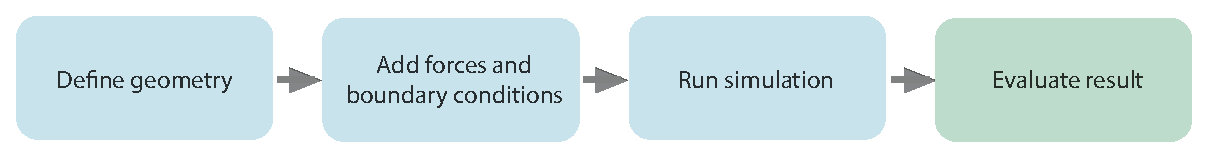
\includegraphics[width=310pt]{graphics/conventional-cycle.eps}
  \caption{Conventional simulation cycle}
  \label{fig:conventional-cycle}
\end{figure}

\begin{figure}
  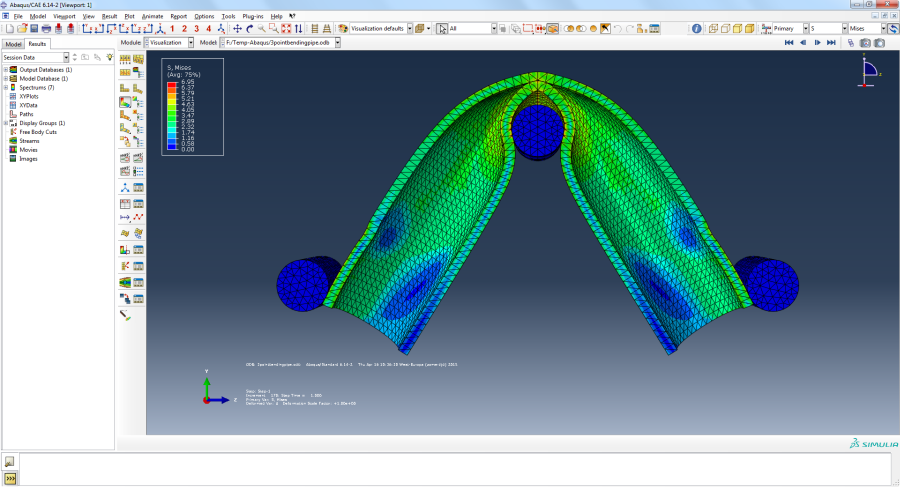
\includegraphics[width=350pt]{graphics/abaqus.png}
  \caption{User interface of conventional analysis software (ABAQUS)}
  \label{fig:abaqus}
\end{figure}

\section{Geometry-based tools for architects}
\subsection{History}
\begin{figure}
  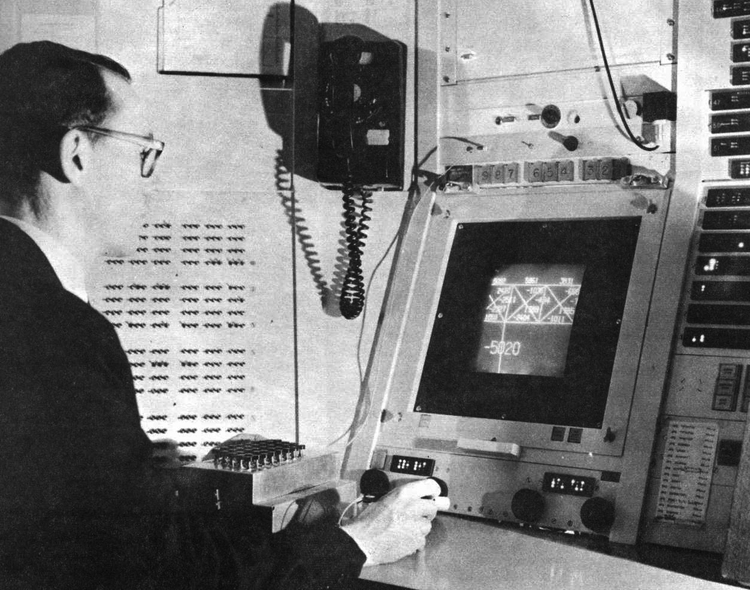
\includegraphics[width=350pt]{graphics/sketchpad.jpg}
  \caption{Sketchpad - the first CAD tool}
  \label{fig:sketchpad}
\end{figure}
The first computer-aided design (CAD) tool, Sketchpad \cite{Aish2005}, was developed by Ivan Sutherland at MIT in 1963. The revolutionary feature of Sketchpad was a real-time representation of the geometry on the display. The geometry could be modified with the use of a new input device, a light pen. The light pen enabled a complete interaction loop between the computer and the designer. The software supported complex relationships between graphical elements; for example, a line could be defined by its relationship to other graphical objects, i.e., perpendicular to, parallel to, same length, etc. Sutherland envisioned that designers would first create a rough sketch of the design, and then, as the design matured, apply constraints to the graphical objects to obtain a more detailed and precise design. 

CAD tools, in the form of 2D drafting tools, first became widely affordable and accessible in the 1980s \cite{Aish2005}. Unfortunately, the subsequent 2D drafting software failed to capture Sutherland’s original intention of using the computer as a creative design tool, as it did not include a constraint model. 

\subsection{Present day}
Many different geometric modeling tools are currently available to designers. For instance, parametric modelers have successfully captured some of Sutherland’s ideas in terms of constraint models. 

The Rhinoceros 3D software \cite{Rhino}, which is a NURBS  modeler, can be combined with the Grasshopper plug-in \cite{Grasshopper} to enable a visual programming environment. The software developer Autodesk has also launched a parametric modeling tool named Dynamo \cite{Dynamo} that has similar features.

In Grasshopper, the designer can connect a slider to a parameter, e.g., the width or curvature of a model, and the geometry then updates in real time as the sliders are manipulated. This enables complex shapes and forms to be generated and manipulated, allowing the designer to explore the parametric design space. 

Grasshopper supports many plug-ins that can be combined with one another. For example, Karamba \cite{Karamba} can be used to provide structural performance feedback within the parametric modeler. 

\section{Existing conceptual design tools}

\textit{``Geometry and algorithms can exist in the abstract, but to be of any practical significance, to become a design tool which can be used by designers, then these have to be encapsulated in an executable form, as working software...''} - Robert Aish \cite{Shea2005}

A number of different conceptual design tools exist. In the following, they have been divided into categories depending on the computational methods that they employ.

\subsection{Real-time analysis tools}

\begin{figure}
  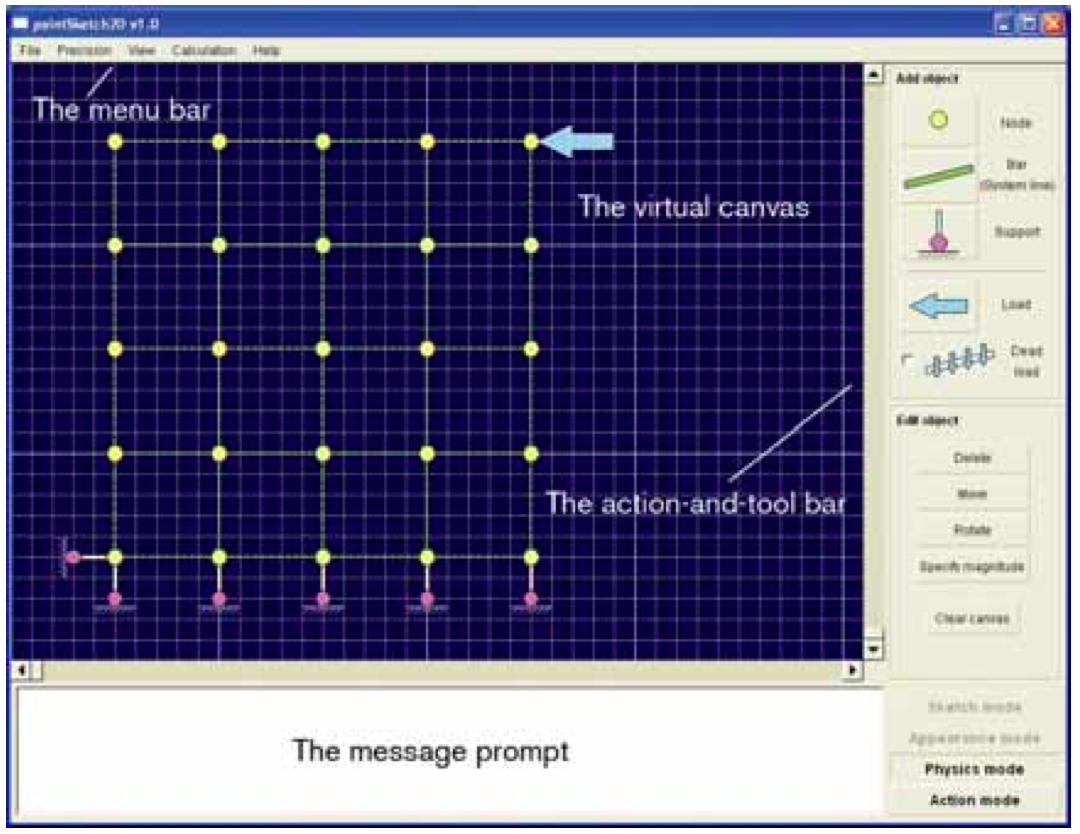
\includegraphics[width=350pt]{graphics/pointsketch.png}
  \caption{The software tool PointSketch}
  \label{fig:pointsketch}
\end{figure}

This type of conceptual design tool makes use of simple mathematical models to provide users with real-time feedback from structural analysis. A number of such tools have been developed; the first two, named Pointsketch \cite{Olsson2006} (see Figure \ref{fig:pointsketch}) and Arcade \cite{martini2008new}, were developed in parallel and released in 2006. Using these software tools, users can create structural models using mouse and keyboard input. Forces can then be applied to the models, and the results are visualized in real time. 

The first tools were developed in academia, but industry has always shown an interest in the concept. Autodesk launched a new application in 2011 named ForceEffect \cite{Autodesk2011}, which is available as both a tablet and web application. The application enables designers to analyze and visualize two-dimensional truss structures. The tablet application utilizes a direct manipulation user interface style whereby users can make changes to the model by directly touching the objects. The commercial finite element (FE) software SAP2000 \cite{sap2000} launched a live model feature in 2012. This feature enables real-time feedback from deformations and forces applied to truss structures \cite{clune2012object}.

Recently, an interactive physics engine was developed to create a game-inspired user experience for design and education \cite{Senatore2015}. This physics engine has been used to create an interactive game called Catastrophe, which aims to teach users which elements are critical to system stability through play.

\subsection{Graphic statics tools}

\begin{figure}
  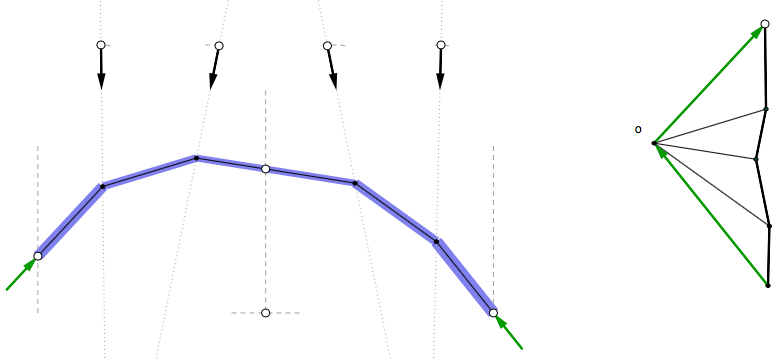
\includegraphics[width=330pt]{graphics/equilibrium.png}
  \caption{The interactive graphic statics software Equilibrium \cite{Block}}
  \label{fig:equilibrium}
\end{figure}

Multiple graphic statics computational design tools have been developed; they make use of the simplicity of graphic statics to allow the computations to run in real time. The first such application was ActiveStatics \cite{ActiveStatics}, a web-based tool that allows users to explore graphic statics. The focus of this tool is on teaching how graphic statics works, and extensive examples are available. A very similar version, named Equilibrium \cite{Block}, was later developed (see Figure \ref{fig:equilibrium}). A similar design tool that makes use of a particle-spring system for computations is CADenary \cite{CADenary}.

\subsection{Interactive optimization design tools}

\begin{figure}
  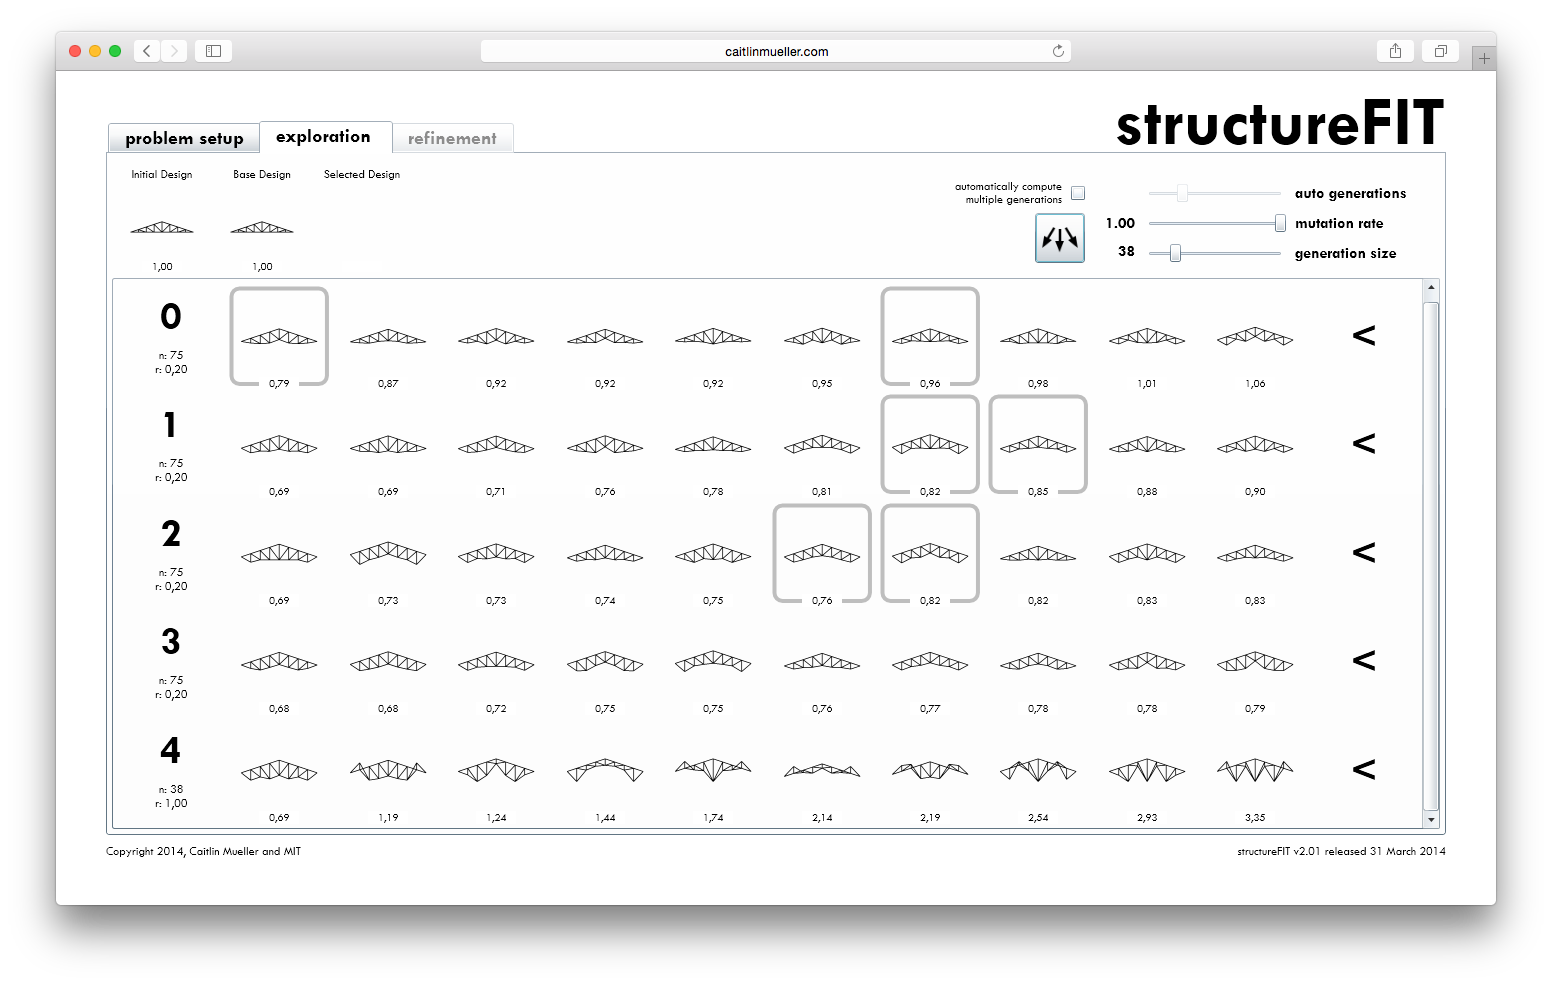
\includegraphics[width=350pt]{graphics/structurefit.png}
  \caption{Screenshot of StructureFIT}
  \label{fig:structurefit}
\end{figure}

Genetic algorithms can easily be used for interactive optimization in which users can intervene in the selection process and direct the population in the desired direction. Such applications have been developed for conceptual structural design to allow the generation and analysis of simple structures. One such tool is von Buelow’s interactive evolutionary design tool \cite{VonBuelow2008}, which supports both 2D and 3D structures.

A similar tool, developed as a web application, is named StructureFIT \cite{Mueller2013, Mueller2015} (see Figure \ref{fig:structurefit}). This software tool has a direct manipulation mode whereby users can further explore the generated structures by moving nodes and observing an updated relative performance index in real time. Another version of this tool, named Stormcloud \cite{Danhaive2015}, has been developed for Grasshopper \cite{Grasshopper}.

\subsection{Topological optimization design tools}
Two other applications that were developed in academia for design exploration through the use of topological optimization are ForcePad \cite{Lindemann2004} (see Figure \ref{fig:forcepad}) and TopOpt \cite{Aage2013}. In these two applications, a 2D geometry is modeled using conventional drawing tools, a metaphor for ``drawing with stiffness.’’ Topological optimization is then performed on the geometry, and the resulting optimized shape is visualized. These applications also have an interactive mode whereby forces can be manipulated and the resulting stresses updated in real time.

\begin{figure}
  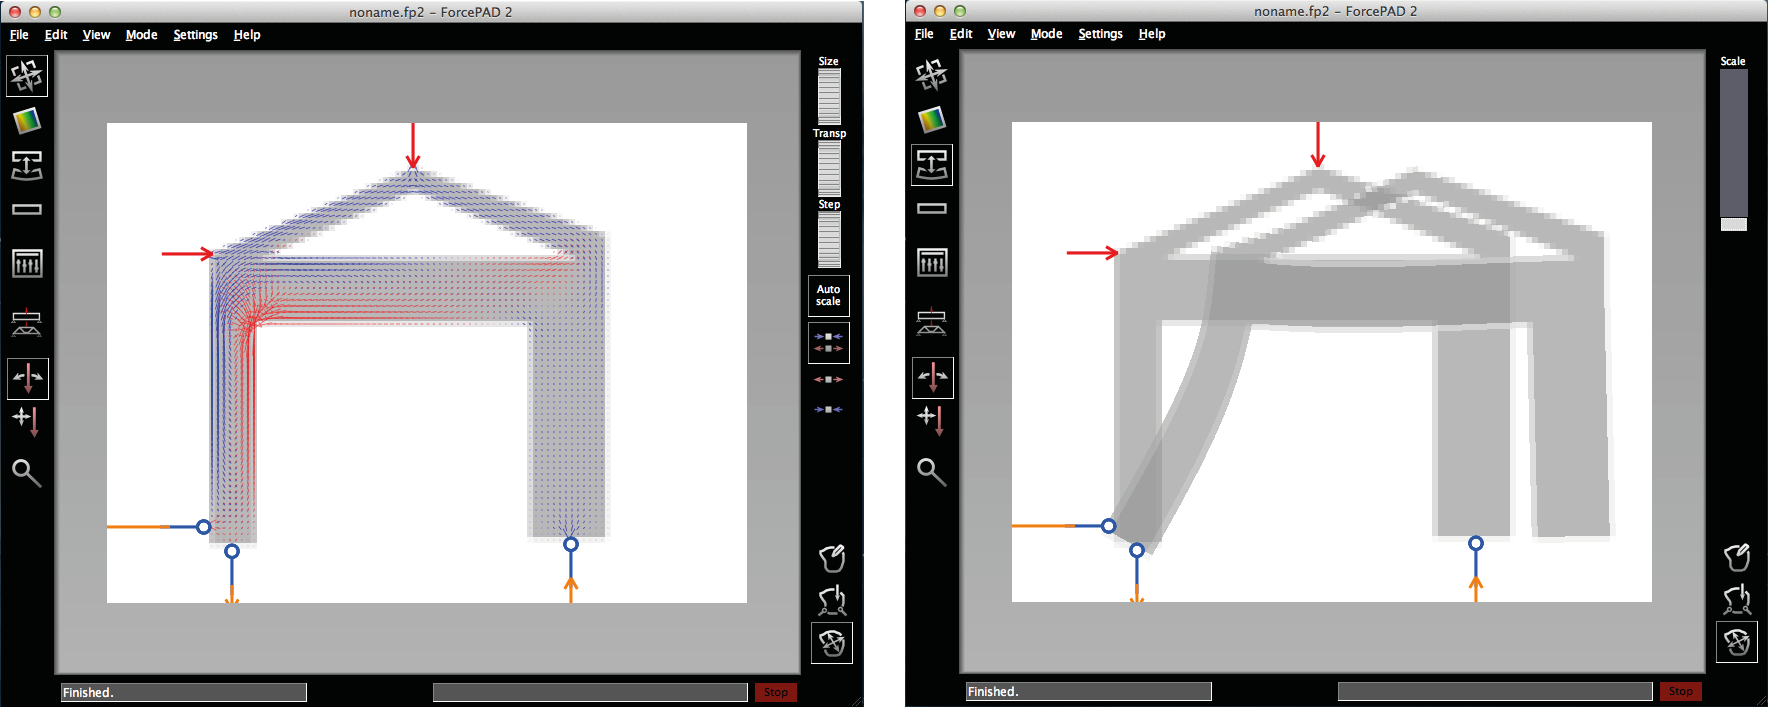
\includegraphics[width=350pt]{graphics/forcepad.png}
  \caption{Software tool ForcePad}
  \label{fig:forcepad}
\end{figure}

